\documentclass[11pt]{article}
\usepackage{amsfonts}
\usepackage{amsmath}
\usepackage{multicol}
\usepackage[utf8x]{inputenc}
\usepackage{graphicx}
\usepackage{geometry}
\geometry{a4paper, total={170mm, 237mm}, left=20mm, top=20mm}
 
\title{ {\Large \textbf{DÉMONSTRATION AUTOMATIQUE EN COQ}} }
\date{}
\author{Quentin Garchery}

\setlength{\parindent}{0cm}



\usepackage{listings}
\usepackage{color}


\lstdefinelanguage{coq}
{morekeywords={[2]apply,eapply,reflexivity, match, with, end, constr, let, in, forall, change, rewrite, auto, simpl, induction, revert, intro, assumption, split, inversion},
keywordstyle={[2]\color{dkblue}},
sensitive=true,
}
\lstset{emph={Lemma, Theorem, Proposition, Qed, Proof, Inductive, Definition, Fixpoint, Ltac}, emphstyle={\color{mauve}\bf}
}
\definecolor{dkblue}{rgb}{0,0,0.6}
\definecolor{dkgreen}{rgb}{0,0.6,0}
\definecolor{gray}{rgb}{0.5,0.5,0.5}
\definecolor{mauve}{rgb}{0.58,0,0.82}

\lstset{frame=tb,
  language=coq,
  aboveskip=3mm,
  belowskip=3mm,
  showstringspaces=false,
  columns=flexible,
  basicstyle={\small\ttfamily},
  numbers=none,
  numberstyle=\tiny\color{gray},
  keywordstyle=\color{blue},
  commentstyle=\color{dkgreen},
  stringstyle=\color{mauve},
  breaklines=true,
  breakatwhitespace=true,
  tabsize=3
}



\begin{document}




\maketitle
\thispagestyle{empty}

\begin{center}
\normalsize sous la direction de \\

\vspace{3mm}

\begin{multicols}{2}
\large Chantal Keller \\
Maître de Conférences\\
Université Paris-Sud \\

\large Valentin Blot \\
Post-doctorant\\
Université Paris-Sud
\end{multicols}

\vspace{7mm}

\Large{Stage au LRI, Paris-Saclay\\
Université Paris-Sud / CNRS \\}

\vspace{5mm}

\normalsize Mars-Août 2018

\end{center}


\vspace{3cm}


\section{Fiche de synthèse}

\subsection{Contexte général : méthodes formelles}

Les méthodes formelles rassemblent différents logiciels formels qui permettent de formuler des propriétés mathématiques puis de les vérifier. La validité du résultat ne dépend alors que de ce logiciel de vérification. C'est dans ce cadre que G. Gonthier et B. Werner ont prouvé, en Coq, le théorème des quatre couleurs.\\

Les méthodes formelles s'étendent à la preuve de programme: il s'agit alors de vérifier qu'un programme correspond à sa spécification. Cela permet d'augmenter la robustesse et la fiabilité du programme certifié. C'est notamment le cas de Compcert \cite{compcert} qui est un compilateur de code C qui a été certifié en Coq par X. Leroy. L'importance de la correction des logiciels est mise en avant dans le cas des systèmes critiques. En effet, le premier lancement d'Ariane 5 (1996) s'est soldé par un échec dû à un bug logiciel. 

\subsection{Problème étudié}

Parmi ces logiciels formels, on s'intéressera aux assistants de preuves (\ref{assistants}) et aux prouveurs automatiques (\ref{prouveurs}) et plus particulièrement aux interfaces entre un assistant de preuve et différents prouveurs automatiques.  De telles interfaces permettent d'améliorer l'automatisation de l'assistant de preuve considéré. En effet, les preuves générées automatiquement par les prouveurs sont ensuite utilisées pour créer des preuves dans l'assistant de preuve. Cette approche est utilisée par Coqhammer \cite{coqhammer} pour Coq et par Sledgehammer \cite{sledgehammer_manual} pour Isabelle. \\
Pendant mon stage, j'ai travaillé sur SMTCoq qui sert aussi d'interface à différents prouveurs automatiques mais qui a la particularité de reconstruire fidèlement, en Coq, les preuves générées par les prouveurs automatiques. Cette approche permet de vérifier les certificats fournis par les prouveurs et donc d'augmenter la confiance que l'on a dans ces outils.\\

Nous aimerions que le développement à l'aide de cette automatisation soit adapté aux assistants de preuves: les preuves sont modulaires et peuvent reposer sur des lemmes précédemment démontrés. Nous voudrions aussi pouvoir formaliser une théorie en partant des axiomes de celle-ci puis démontrer automatiquement de nouvelles propriétés de cette théorie.

\subsection{Contribution proposée}

Pendant mon stage, je me suis attaché à améliorer l'expressivité de SMTCoq de ce point de vue là. J'ai donc donné la possibilité à l'utilisateur de rajouter au contexte courant des lemmes (ou des axiomes) en forme prénexe. Ces lemmes sont ensuite traduits pour pouvoir être envoyés à un prouveur automatique. Ceux-ci fournissent alors un fichier de certificat et j'ai modifié la représentation SMTCoq de ces certificats pour y ajouter l'instanciation des lemmes. Cet aspect est original : la technique d'encodage des instanciations utilisée (\ref{processing_forallinst}) permet d'alléger la suite de la vérification. Enfin, j'ai automatisé l'instanciation de ces lemmes dans la preuve.


\subsection{Arguments en faveur de la validité de la contribution}

En plus des tests déjà présents dans SMTCoq initialement, le code final passe d'autres tests pour s'assurer du gain d'expressivité dû au rajout des lemmes et des quantificateurs. J'ai par exemple pu vérifier des propriétés, automatiquement et dans Coq, en théorie des groupes, dans une théorie formalisant les listes d'entiers, sur des fonctions définies récursivement, etc. \\ 

D'autre part, ma contribution respecte le principe sceptique de SMTCoq (\ref{sceptique_autarcique}), le développement et le calcul sont faits principalement en Ocaml, en dehors de l'assistant de preuve. Cet aspect donne une meilleure robustesse à SMTCoq face aux changements internes des prouveurs automatiques.


\subsection{Bilan et perspectives}\label{persp}

Un des buts que l'on souhaite poursuivre est de certifier le logiciel de vérification Why3 \cite{why3_intro}. Puisque Why3 utilise des prouveurs automatiques, il faut alors pouvoir certifier les démonstrations faites par ces prouveurs. Ce sujet est lié à celui de ma thèse intitulée "Certification de la génération et la transformation d'obligations de preuves" et encadrée par Claude Marché, Chantal Keller et Andrei Paskevitch. À cette occasion, j'utiliserai SMTCoq et je profiterai de l'amélioration de son expressivité dûe à mon stage. Je pourrai l'améliorer encore afin d'accepter des quantificateurs dans n'importe quelle position dans la formule.\\
L'expressivité peut également être améliorée en considérant les termes concrets du type des propositions dans Coq en plus de ceux du type des booléens. \\
On pourrait aussi utiliser des méthodes de machine learning pour sélectionner les lemmes à envoyer au prouveur automatique comme c'est fait dans Coqhammer et Sledgehammer \cite{hol_selector, coqhammer}. L'avantage étant qu'avec des lemmes pertinents et en petit nombre le prouveur automatique trouve plus rapidement et plus souvent la preuve du théorème en question.


\newpage
\section{Logiciels utilisés}

\subsection{Assistants de preuve}\label{assistants}

Les assistants de preuves tels que Coq sont des outils puissants qui permettent d'exprimer des théorèmes complexes puis de les vérifier de manière interactive. Ils proposent à un utilisateur de formuler son problème puis de le démontrer, le rôle principal de l'assistant de preuve étant alors de vérifier que la preuve fournie est correcte. Pour une propriété donnée, l'utilisateur doit donc fournir une preuve parfaitement rigoureuse et exhaustive de la propriété ce qui peut rendre le processus de vérification long et fastidieux. La confiance accordée à ces outils dépend de la compréhension que l'on peut avoir dans son noyau, étant donné que c'est la partie sur laquelle repose la vérification. Cette compréhension est facilitée lorsque l'implantation de la logique de ce noyau est de taille réduite. 

\subsection{Prouveurs automatiques}\label{prouveurs}

Les prouveurs automatiques, quant à eux, ne demandent pas de preuves de la part de l'utilisateur. L'effort de certification est alors réduit à la formalisation du problème et dans certains cas le prouveur donne une trace de son exécution appelée certificat. En contrepartie, la logique d'un prouveur automatique est plus limitée et/ou la réponse en temps fini n'est pas garantie.

\subsection{Coq}

L'assistant de preuve que nous utiliserons est Coq, la logique de son noyau se fonde sur le calcul des constructions inductives \cite{coq_intro}. 
On supposera connu la syntaxe et la sémantique de Coq, y compris le langage des tactiques. La partie \ref{coq} introduit deux techniques d'utilisation de Coq.

\subsection{zChaff et veriT}

Les prouveurs automatiques que nous utiliserons sont : 
\begin{itemize}
    \item zChaff, un SAT-solveur
    \item veriT, un SMT-solveur (voir \ref{smt})
\end{itemize}


\subsection{SMTCoq}
 SMTCoq est un \textit{plugin} pour Coq qui utilise différents prouveurs automatiques. C'est un outil modulaire dans le sens où il est possible de rajouter d'autres prouveurs automatiques, ceux-ci n'étant pas nécessairement du même type (SAT/SMT-solveurs) et n'ayant pas nécessairement le même format d'entrée ni le même format de sortie. \\

SMTCoq est actuellement développé par Chantal Keller en collaboration avec l'université de l'Iowa. \\

Pendant ce stage j'ai travaillé sur SMTCoq, j'ai notamment eu l'occasion de modifier le code du projet.

\newpage

\section{Techniques de preuves en Coq} \label{coq}

On donne ici deux techniques de preuves en Coq qui peuvent être combinées : la réflexion calculatoire et la réification. Ces techniques sont au coeur du fonctionnement de SMTCoq.



\subsection{Réflexion calculatoire}

La preuve par réflexion repose sur la convertibilité de deux termes: deux termes sont convertibles lorsqu'ils se réduisent vers un même terme. \\
Aussi, à chaque nouvelle instance de Definition ou Fixpoint, la nouvelle constante qui est définie est convertible avec sa définition. Prenons l'exemple des formules conjonctives : 

\begin{lstlisting}[frame=single]
Inductive AndTree :=
  And (_ _: AndTree)
| Bool (_ : bool).
\end{lstlisting}

et définissons un type inductif qui donne son évaluation : 

\begin{lstlisting}[frame=single]
Inductive Evaluation : AndTree -> bool -> Prop :=
  EvalBool b :
    Evaluation (Bool b) b
| EvalAnd b1 b2 b3 t1 t2 :
    Evaluation t1 b1 -> Evaluation t2 b2 -> b1 && b2 = b3 ->
    Evaluation (And t1 t2) b3.
\end{lstlisting}
$Evaluation \, t \, b$ signifie que l'arbre $t$ s'évalue en un booléen $b$. Cette définition suit la définition des formules conjonctives. En effet, il y a bien deux cas, $EvalBool$ pour les feuilles de l'arbre et $EvalAnd$ pour les noeuds.  
On peut alors faire des preuves sur les éléments de ce type inductif : 
\begin{lstlisting}[frame=single]
Definition t := And (And (Bool true) (Bool false)) (And (Bool true) (Bool true)).

Lemma Eval_t_false : Evaluation t false.
Proof.
  eapply EvalAnd ; [
    eapply EvalAnd ; [ apply EvalBool | apply EvalBool | reflexivity ]
  | eapply EvalAnd ; [ apply EvalBool | apply EvalBool | reflexivity ]
  | reflexivity ].
Qed.
\end{lstlisting}

Cependant, plutôt que d'utiliser un prédicat qui prend une formule conjonctive $t$ et un booléen $b$ et qui vérifie que $t$ s'évalue en $b$, on peut utiliser une fonction récursive qui calcule l'évaluation et combiner cette fonction récursive avec le prédicat de l'égalité. On peut montrer que les deux définitions sont bien équivalentes.  
\begin{lstlisting}[frame=single]
Fixpoint evaluation (t : AndTree) :=
  match t with
    And t1 t2 => evaluation t1 && evaluation t2
  | Bool b => b
  end.
  
Proposition Eval_eq_eval t b :
  Evaluation t b <-> evaluation t = b.
  
\end{lstlisting}

L'avantage de cette nouvelle définition de l'évaluation est que, grâce à la convertibilité de $evaluation$ avec sa définition, on a une preuve triviale de la propriété.
\begin{lstlisting}[frame=single]
Lemma eval_t_false : evaluation t = false.
Proof.
  reflexivity.
Qed.
\end{lstlisting}

Ce fonctionnement peut être exploité pour construire des preuves qui reposent sur un calcul effectué en Coq. 


\subsection{Réification}

\subsubsection{\textit{Embeddings}}

La réification est le fait de passer d'un \textit{shallow-embedding} à un \textit{deep-embedding}. \\

Dans le cas du \textit{deep-embedding}, un terme est représenté dans un nouvel AST ce qui met en évidence sa structure. À l'inverse, un \textit{shallow-embedding} du même terme est traduit directement vers sa valeur dans le langage cible. \\

Reprenons l'exemple des formules conjonctives et considérons la formule $ u = (b_1 \,\&\, b_2) \,\&\, (b_3 \,\&\, b4)$. À l'instar de la section précédente, le \textit{deep-embedding} de $u$ est donné dans le type $AndTree$ :
\[And\,(And\,(Bool\,b1)\,(Bool\,b2))\,(And\,(Bool\,b3)\,(Bool\,b4))\] 
et son \textit{shallow-embedding} peut être donné en utilisant la fonction Coq $andb$ notée $\&\&$ : 
\[(b1\,\&\&\,b2)\,\&\&\,(b3\,\&\&\,b4) \]\,

Dans la suite, on s'intéresse au problème de mettre des formules booléennes conjonctives en forme de peigne. Avec $b_1, b_2, b_3, b_4$ des termes de type $bool$, on veut, par exemple, pouvoir passer de : 
\begin{center}
$ u = (b_1 \,\&\&\, b_2) \,\&\&\, (b_3 \,\&\&\, b4)$ \hspace{1cm} à   \hspace{1cm}  $u' = b_1 \,\&\&\, (b_2 \,\&\&\, (b_3 \,\&\&\, b4)). $
\end{center}

Pour cela, on a besoin de récupérer la structure du booléen $u$, c'est l'étape de réification. Il s'agit donc de construire, à partir de $u$, un terme du type $AndTree$ qui a la même structure que $u$. \\

\subsubsection{Méthodes}
Il n'est pas possible d'écrire en Coq une fonction qui détermine la forme conjonctive d'un argument booléen. En effet, le type $bool$ n'ayant que deux constructeurs ($true$ et $false$), inspecter par \textit{pattern-matching} nous donnera un de ces deux constructeurs.\\

Une solution est d'étudier la structure du terme en question à partir de sa représentation Ocaml sous-jacente. C'est l'approche utilisée par SMTCoq. \\

Il est aussi possible d'utiliser des tactiques qui renvoient un terme. Dans le cas des formules conjonctives, on définit :

\begin{lstlisting}[frame=single]
Ltac reify A :=  match A with
  | andb ?X ?Y => let rx := reify X in
                    let ry := reify Y in
                    constr:(And rx ry)
  | ?X => constr:(Bool X) end.

\end{lstlisting}

Le terme $u = (b1\,\&\&\,b2)\,\&\&\,(b3\,\&\&\,b4)$ réifié donne bien 
\[And\,(And\,(Bool\,b1)\,(Bool\,b2))\,(And\,(Bool\,b3)\,(Bool\,b4))\] 
et on notera que l'évaluation de ce nouveau terme est égale à $u$.



\subsubsection{Intérêt et exemple d'utilisation}

L'intérêt de la réification est que la structure du terme réifié est mise en évidence. Il devient alors possible de manipuler explicitement cette structure. \\

Par exemple, sur le type $AndTree$, il est possible de définir une fonction $peigne$ qui renvoie l'arbre en argument mis sous forme de peigne. Le théorème de correction de cette fonction établit que 
\[ \forall t \in AndTree, \, evaluation \, (peigne \, (t)) = evaluation (t) \]

En combinant ce résultat avec le procédé de réification, on peut définir une tactique $peignify$ qui met les formules conjonctives en forme de peigne. Cette tactique permet par exemple de démontrer le lemme suivant : 

\begin{lstlisting}[frame=single]
Lemma peigne4 b1 b2 b3 b4:
  (b1 && b2) && (b3 && b4) = b1 && ((b2 && b3) && b4).
Proof.
  peignify. reflexivity.
Qed.
\end{lstlisting}
Cette preuve a un contenu calculatoire : le calcul de la fonction $peigne$ sur la réification du terme $u$ de type $bool$. Pour le code complet de cette partie, voir l'annexe \ref{annexe_peigne}, la preuve de correction est inspirée de \cite{coq_intro}, \textbf{3.3}.


\newpage
\section{Fonctionnement d'un prouveur automatique} \label{fonctionnement_prouveurs}

\subsection{SMT-LIB}\label{smt-lib}

SMT-LIB est un langage qui a vocation à être un format d'entrée commun avec différents solveurs SMT qui sont un cas particulier des prouveurs automatiques, voir la section suivante. Ce langage offre un cadre commun pour faire des comparaison de solveurs SMT. La définition du langage \cite{smtlib} donne des indications sur la sémantique que doivent avoir certaines constructions du langage.\\

Par exemple, pour le fichier texte $lia5.smt2$ suivant, les prouveurs automatiques doivent vérifier si il existe deux entiers $x$ et $y$ tels que $ ((x + y \leq -3 \wedge y \geq 0) \vee x \leq -3) \wedge x \geq 0$.    
\begin{lstlisting}[frame=single]
(set-logic QF_LIA)
(declare-fun x () Int)
(declare-fun y () Int)
(assert (and (or (and (<= (+ x y) (- 3)) (>= y 0)) (<= x (- 3))) (>= x 0)))
(check-sat)
(exit)
\end{lstlisting}

\subsection{Solveurs SMT} \label{smt}

Expliquons le fonctionnement d'une version simplifiée de l'algorithme DPLL \cite{dpll}. Nous ne considèrerons que la théorie LIA, c'est-à-dire qu'en plus des connecteurs logiques, la théorie contient les entiers et les symboles d'addition, de soustraction et d'inégalité. On prend en exemple la formule de la section précédente. L'algorithme commence par identifier les sous-formules spécifique à la théorie LIA qu'on appelera atomes. Dans notre exemple cela revient à poser
\begin{align*}
  a &= (x + y \leq -3)\\
  b &= (y \geq 0)\\
  c &= (x \leq -3) \\
  d &= (x \geq 0)
\end{align*}
et à chercher si la formule  $((a \wedge b) \vee c) \wedge d$ est satisfiable. Cette étape peut être suivie par une transformation de Tseitin (voir \ref{tseitin}) afin d'obtenir un problème en CNF. \\

Ensuite l'algorithme DPLL répète les étapes suivantes :
\begin{itemize}
\item Appeler un SAT-solveur sur l'ensemble des formules (dans l'exemple on commence avec une seule formule). Si ce n'est pas satisfiable alors l'algorithme répond que le problème n'est pas satisfiable.
\item Sinon, le SAT-solveur donne une instanciation qui satisfait toutes les formules. Dans l'exemple, une telle instanciation pourrait être :
  $a \wedge \neg b \wedge c \wedge d$
ce qui signifie que toutes les variables booléennes sont à $true$ sauf $b$ qui est à $false$.
\item Vérifier que l'instanciation est valide dans les théories. Si c'est le cas, l'algorithme renvoie que le problème est satisfiable.
\item Sinon, rajouter la négation de l'instantiation à la liste des formule et recommencer. C'est le cas de notre exemple au premier tour de boucle. En effet, il n'est pas possible, dans la théorie LIA, d'avoir à la fois $x \leq -3$ et $x \geq 0$. À la fin de cette étape, le problème est donc ramené à la satisfiabilité des deux formules suivantes:
  \begin{align*}
    ((a \wedge b) \vee c) \wedge d \\
    \neg a \vee b \vee \neg c \vee \neg d
  \end{align*}


\end{itemize}

Cet algorithme termine puisque qu'à chaque tour de boucle une nouvelle instanciation des atomes n'est plus possible et qu'il y a un nombre fini de telles instanciations. \\

Lorsqu'on appelle un prouveur automatique sur un fichier SMT-LIB (\ref{smt-lib}), si l'ensemble des assertions est satisfiable, le prouveur renvoie $sat$. Si l'ensemble des assertions n'est pas satisfiable, le prouveur renvoie $unsat$ et fournit un fichier de certificat qui explique pourquoi ce n'est pas satisfiable. 

\subsection{veriT}

veriT est un SMT-solveur qui prend un fichier SMT-LIB en entrée. 

Les certificats de veriT sont constitués d'une liste de règle de la forme :\\
\textit{id:(typ (clause) dep)}\\
où \textit{id} est un entier qui identifie la règle, \textit{type} est le type de la règle,
\textit{clause} est le résultat de la règle et \textit{dep} liste toutes les dépendance de la règle. \\

Par exemple, la règle suivant est une règle de résolution qui dépend des règles 0 et 1 et qui produit la clause vide : \\
\textit{2:(resolution () 0 1)} \\


A FAIRE : schéma d'un certificat verit, explication du certificat, comment on arrive à la clause vide


\subsection{Utilisation par SMTCoq}

SMTCoq utilise les prouveurs automatiques comme des boites noires qui résolvent des problèmes logiques. Plus précisément, SMTCoq intéragit avec un prouveur automatique en traduisant le problème dans un format reconnu par celui-ci puis en interprétant sa réponse. Ce fonctionnement est un des intérêts de l'approche sceptique comme expliqué dans la partie suivante.


\newpage 
\section{Présentation de SMTCoq}

\subsection{SMTCoq, une interface sceptique entre Coq et les prouveurs automatiques}\label{sceptique_autarcique}

Pour améliorer l'automatisation de Coq et y intégrer l'utilisation de prouveurs automatiques, il y a principalement deux approches.

\begin{multicols}{2}
\begin{center}
Approche autarcique\\
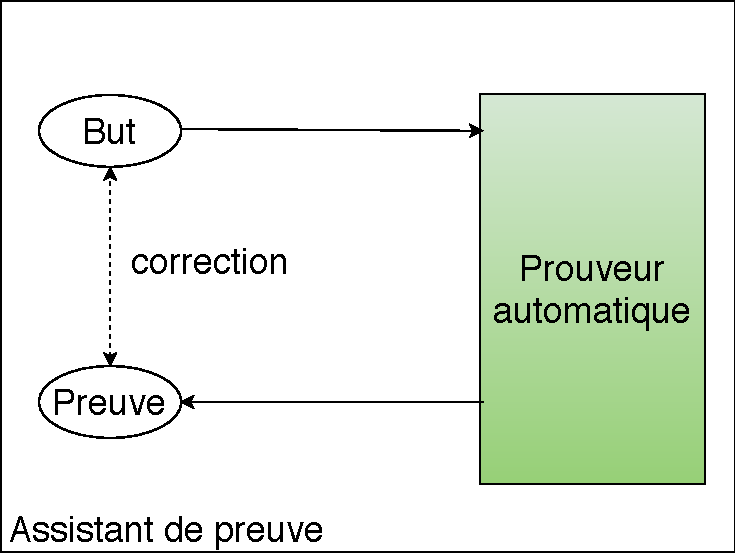
\includegraphics[height=5cm]{1_Autarcique.pdf}\\
Approche sceptique\\
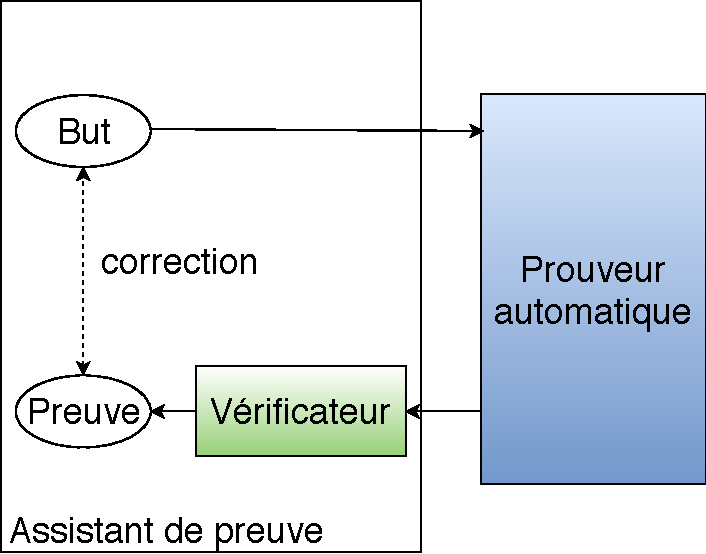
\includegraphics[height=5cm]{2_Sceptique.pdf}\\

\end{center}
\end{multicols}

L'approche autarcique consiste à vérifier le code du prouveur automatique à l'intérieur de l'assistant de preuve. L'avantage de cette méthode est qu'une fois cette vérification faite, on sait que chaque appel du prouveur automatique nous renverra une preuve correcte. \\

Dans l'approche sceptique, le certificat renvoyé par le prouveur automatique est vérifié à chaque appel de celui-ci. D'un côté cela signifie que la complétude du système n'est pas garantie : certains buts valides ne sont pas démontrés lorsque le prouveur automatique renvoie un certificat erroné ou que la reconstruction de la preuve par SMTCoq contient un \textit{bug}. D'un autre côté, cette approche ne fige pas l'implantation du prouveur automatique puisque ce n'est pas son code qui est vérifié mais sa sortie. Un autre avantage est que l'effort de certification est plus restreint : pour un certificat fixé, il faut vérifier que celui-ci correspond bien à une preuve du but.\\

SMTCoq a une approche sceptique de la vérification des prouveurs automatiques.

\subsection{Fonctionnement de SMTCoq}

\subsubsection{Amélioration de l'automatisation}

SMTCoq définit des tactiques Coq, une par prouveur automatique : \textit{zchaff} et \textit{verit}. \\


\begin{center}
    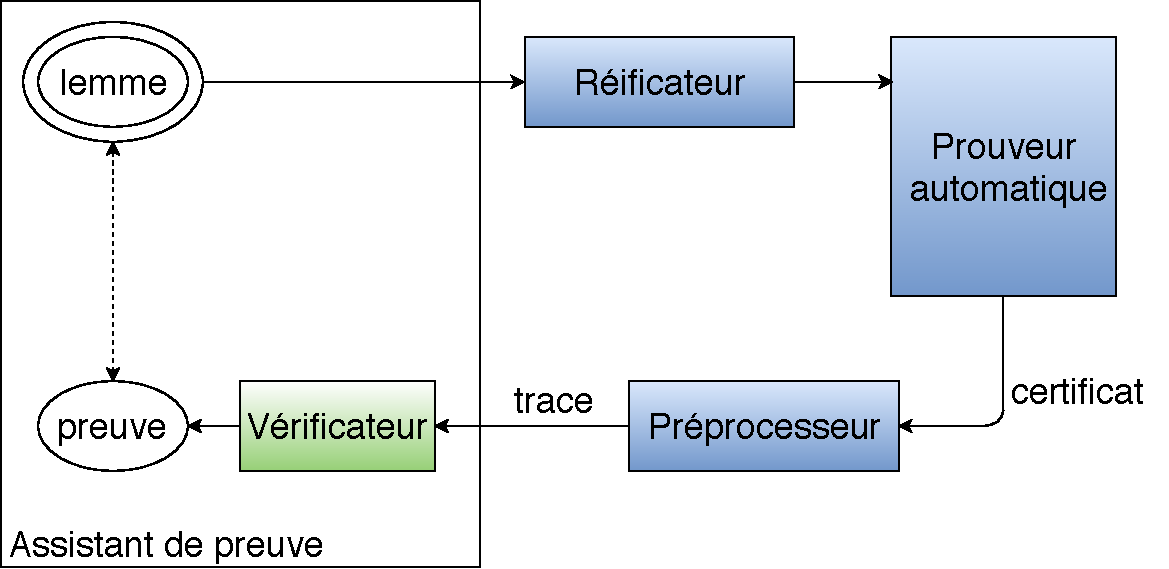
\includegraphics[height=5cm]{Automatisation.pdf}
\end{center}

La première étape est la réification, le lemme est traduit dans l'AST des formules acceptées par SMTCoq. Le prouveur automatique est appelé à partir de cet AST. En cas de succès de ce prouveur, on obtient un certificat de preuve. 
Il s'agit ensuite de rejouer ce certificat en Coq, on utilise pour cela le vérificateur de SMTCoq. Il faut donc mettre le certificat dans une forme adaptée qu'on appelle trace. Le pré-processeur effectue une étape de \textit{parsing} du certificat qui se souvient des sous-formules déjà rencontrées (\textit{hash-consing}) à l'aide de \textit{hash tables}.  Il y a aussi une étape d'adaptation de ces certificats. En effet, les prouveurs automatiques peuvent parfois ne pas mentionner une étape de la preuve qu'il faut alors construire. De plus, il faut pouvoir adapter les certificats à fournis par le prouveur automatiques qui peuvent reposer sur une logique différente de celle de Coq. \\

Ces tactiques permettent à l'utilisateur Coq de profiter de l'automatisation de différents prouveurs.\\

Les prouveurs automatiques fournissent un certificat uniquement dans le cas où le problème n'est pas satisfiable (\ref{smt}). Pour utiliser ce fonctionnement, SMTCoq envoie la négation du but au prouveur automatique. On s'attend alors à obtenir $unsat$. Si c'est le cas on a montré que la négation du but implique la clause vide. Autrement dit, on a une preuve de la double négation du but. SMTCoq ne traitant que les cas où les domaines des variables sont décidables, on récupère une preuve de but initial.


\subsubsection{Amélioration de la confiance}

Dans la suite on s'attachera principalement à développer l'aspect automatisation de Coq mais SMTCoq propose également une commande de reconstruction d'une preuve effectuée par un prouveur automatique.

\begin{center}
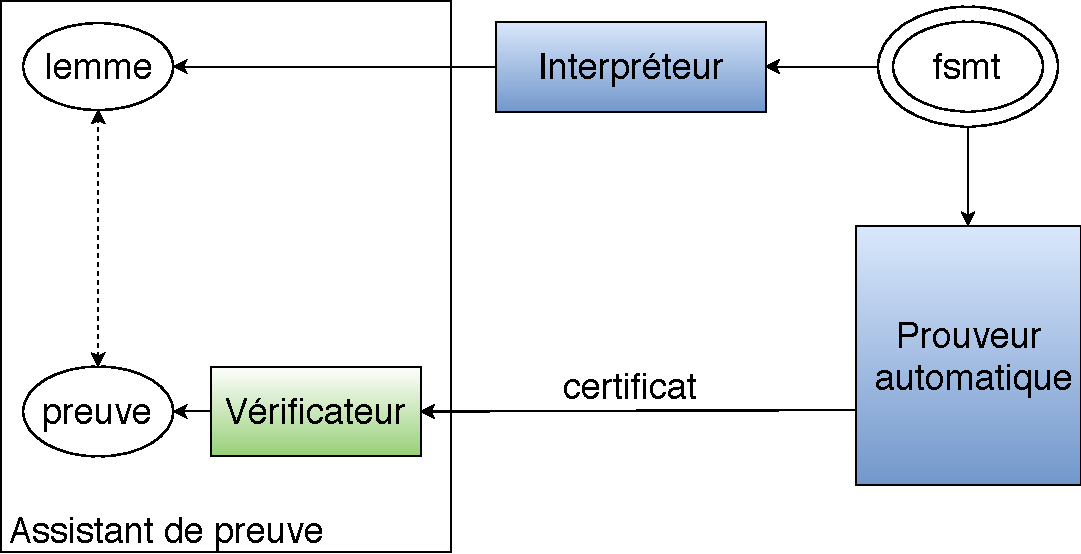
\includegraphics[height=5cm]{Confiance.pdf}
\end{center}

Cette commande prend en paramètre un fichier 'fsmt' décrivant le lemme (typiquement écrit en SMT-LIB) et le certificat fourni par un prouveur automatique. Le lemme Coq est reconstruit à l'aide de l'interpréteur de SMTCoq et la preuve est reconstruite grâce au vérificateur. Une fois la reconstruction faite, la vérification que la preuve correspond bien au lemme est laissée à Coq. \\

Puisqu'un nouveau lemme Coq est créé, l'utilisateur peut vérifier que c'est bien le but qu'il voulait prouver. Ainsi, la confiance dans les prouveurs automatiques est améliorée: on peut vérifier la réponse du prouveur.


\subsubsection{Cas d'application de SMTCoq}

Dans les deux cas, les formules acceptées sont les formules logiques propositionnelles en forme prénexe. Les domaines de quantifications doivent aussi être décidables. La logique est étendue avec les combinaisons des théories suivantes : arithmétique linéaire sur $\mathbb{Z}$, égalité et fonctions non-interprétées, auxquelles s'ajouteront la théorie des vecteurs de bits et théorie des tableaux. 

\subsection{Utilisation de SMTCoq}

\subsubsection{La tactique verit}

SMTCoq définit une nouvelle tactique, appelée dans Coq par \textit{verit}, qui permet de résoudre automatiquement les buts dans les booléens en forme prénexe. On reprend l'exemple de la partie \ref{fonctionnement_prouveurs}.


\begin{lstlisting}[frame=single]
Lemma lia5 : 
  forall x y,
    negb ( ((x+y <=? - (3)) && (y >=? 0) || (x <=? - (3))) && (x >=? 0)).
Proof.
    verit.
Qed.
\end{lstlisting}

La tactique commence par introduire les variables quantifiées universellement en tête de formule (ici c'est $x$ et $y$) puis s'attend à ne pas avoir d'autres quantificateurs. C'est ensuite la négation de la formule qui est envoyée à veriT. La reconstruction de la preuve ne peut avoir lieu que si veriT renvoie $unsat$ ainsi qu'un fichier de certificat.

\subsubsection{La commande de reconstruction}

La commande $Verit\_Theorem$ nous permet de créer un terme Coq à partir du certificat fourni par veriT appelé sur $lia5.smt2$. On obtient alors le terme Coq $lia5$ : \\

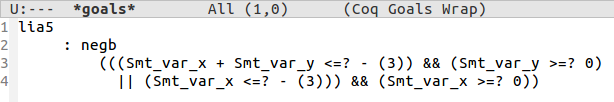
\includegraphics[height=2cm]{checklia5.png}

On notera que c'est bien la négation de la formule énoncée dans le fichier SMT-LIB. 


\newpage
\section{Certificats et vérificateur}

\subsection{Interpétation des certificats}

La tactique \textit{verit} interprète le fichier de certificat \textit{tcertif} fourni par le prouveur automatique en un terme Coq \textit{ccertif} ce qui permet de construire une preuve du but initial. \\

\begin{center}
\begin{tabular}{ |c||c|c|c| } 
 \hline
 Format & Fichier texte & Code Ocaml & Code Coq \\ 
 \hline
 Appellation & \textit{tcertif} & \textit{ocertif} & \textit{ccertif} \\ 
 \hline
 Composant & \textit{trule} & \textit{orule} & \textit{crule} \\ 
 \hline
\end{tabular}
\end{center}

Cette interprétation passe par une étape intermédiare \textit{ocertif} écrite en Ocaml. Cette étape a plusieurs avantages. Déjà, elle permet d'utiliser les outils de parsing du fichier de certificat (ocamllex, ocamlyacc). Par ailleurs, en utilisant la représentation Ocaml des termes Coq, la traduction d'un \textit{ocertif} en un \textit{ccertif} est immédiate. Enfin, les \textit{ocertif} sont définis dans un format facilement manipulable ce qui permet d'appliquer des adaptations (\ref{processing_forallinst}), des simplifications (\ref{regroupement}) ou encore des optimisations (\ref{alloc}).




\subsection{Transformation de Tseitin et hash-consing} \label{tseitin}

\subsubsection{Motivations}

La transformation de Tseitin d'une formule donne une formule equisatisfiable qui est en CNF. L'avantage de cette transformation est que sa complexité est linéaire en temps comme en espace. En comparaison, l'utilisation des lois de de Morgan pour obtenir une formule en CNF a une complexité en pire cas exponentielle. Le principe de cette transformation est d'introduire de nouvelles variables pour toutes les sous-formules ce qui correspond au \textit{hash-consing} qui est fait par SMTCoq. Du côté SMTCoq, l'intérêt est double. D'une part, cela permet de réduire la taille des formules

\subsection{Fonctionnement}

-tables \\
-nouvelles variables\\
Tseitin: exemple, transformation linéaire\\
intérêt dans smtcoq : suivre fidèlement les certificat verit qui sont fait comme ça,
optimisation



 \subsection{Le type inductif \textit{crule}}\label{regroupement}



Une clause contient un $scertif$  qui est représentée par un type somme, chaque constructeur regroupant plusieurs étapes qui peuvent apparaître dans le certificat.\\

A FAIRE : un schéma sur les scertif :  inductive scertif = ImmBuildProj c params $|$ EqTr f1 ... fn f \\

Le constructeur ImmBuildProj par exemple regroupe les règles not\_implies1 et not\_implies2. EqTr est la transitivité de l'égalité : f1 .. fn et f doivent suivre le chéma de la transitivité : par exemple f1 = ~(a1=a2) f2= ~(a2=a3) ... fn=~(an=a{n+1}) et f = (a1 = a{n+1}).\\

\subsection{La fonction récursive $checker$} 
Le vérificateur définit une fonction Coq $checker$ qui est définie récursivement sur son paramètre trace qui est un tableau de clauses et qui maintient un tableau de formules appelées état. À chaque appel de checker, une nouvelle clause est consommée, $checker$ met alors à jour l'état courant.\\

Pour chaque constructeur $X$ de $scertif$ correspond une fonction $schecker$ qui est appelée par $checker$ lorsque le constructeur $X$ est rencontré. $schecker X$ donne une nouvelle formule valide à partir de celles déjà présentes dans l'état (et des tables de hashage, etc). Par exemple le $schecker$ de EqTr f1 ... fn f avec f1 ...fn et f comme ci-dessus donne la tautologie (f1 \/ ... \/ fn \/ f). Les clauses contiennent aussi une position qui indique où enregistrer la nouvelle formule.\\

Enfin $checker$ utilise un paramètre de position. Lorsque tous les calculs de mise à jour de clause sont faits, checker regarde à la position indiquée par l'état et renvoie vrai si la clause est vide à cet endroit et faux sinon.

\subsection{Exemples de certificats et de vérificateurs}
\subsubsection{resolution chains}
C'est simplement une liste de clause.
Le schecker associé fait un fold dessus en appliquant la règle de resolution dessus. Cette règle est refutationnellement complète.

\subsubsection{nor\_certif}
Il implémente la règle $\neg (A_1 \vee A_2 \vee ... \vee A_n) \Rightarrow \neg A_i$

\subsubsection{congruence theory}
Qui implémente les règles de transitivité et de congruence.

\subsection{Calcul de $checker$} \label{alloc}
L'état est représenté par un tableau de taille fixée initialisé avec la négation du but. Si on arrive à en déduire la clause vide alors on aura que la double négation du but est vraie. Puisque le domaine d'étude est décidable, et que les formules prouvées sont sans quantificateur, on a bien construit une preuve du but. \\

A partir de la trace, la fonction $alloc$ calcule le nombre maximum de clauses à retenir à chaque étape du $checker$ (cette valeur est choisie comme la taille du tableau d'état) et assigne une position à chaque clause de la trace pour respecter cette valeur. Les clauses qui ne seront plus utilisées sont libérées, de sorte que les nouvelles clauses peuvent utiliser ces nouveaux emplacements dans l'état. \\

Une trace est représentée par une liste doublement chaînée de clauses, cela permet sa modification en place. Les clauses sont formées d'un $scertif$, de ses paramètres et de la position à modifier. Lors du parcours de la trace, à chaque nouvelle clause, l'état est modifié. Par exemple, la clause $(2, not\_implies1 \, 0)$ modifie la deuxième clause de l'état et prend comme paramètre la clause $0$ de l'état. Cette clause transforme l'état 
\[    [\neg (A \Rightarrow B);  C; D] \quad \text{en} \quad [\neg (A \Rightarrow B);  C; \neg B]. \]
La clause $(0, not\_implies0 \, 0)$ transforme ce nouvel état en $[A; C; \neg B]$. \\


\subsection{Théorème de correction}

Le vérificateur repose sur le théorème de correction suivant :

\[ \forall l \, \forall t. \quad checker \, t = true \quad \Rightarrow \quad interp \, l \]







\newpage
\section{Ajout de quantificateurs}

\subsection{Instanciation de lemmes par veriT}

Considérons le but : \\

A FAIRE : schéma du but : instance1 f (2) = 3 avec comme lemme initial forall x, f (x) = 3 \\

Lorsqu'un lemme en forme prénexe est donné en input, veriT peut instancier ce lemme avec la commande de type FORALLINST. \\

A:(INPUT (forall x, f (x) = 3)) \\
B:(FORALLINST (or (not (forall x, f (x) = 3)) (f (2) = 3))) \\

On remarquera que la commande FORALLINST ne dépend pas de l'input. L'utilisation de la commande B passe par une règle OR puis une règle RESOLUTION : \\ 

C:(OR ( (not (forall x, f (x) = 3)) (f (2) = 3)) B) \\ 
D:(RESOLUTION (f (2) = 3) A C) \\ 

On fera attention ici, que même si ce schéma fait clairement apparaître la dépendance de FORALLINST au théorème donné en A, cette dépendance est perdue dans la suite du certificat. En effet, dans une règle de RESOLUTION qui a plus que 2 dépendances, retrouver le théorème et son instanciation demande, a priori, d'unifier des formules contenues dans une commande FORALLINST et dans une commande input. De plus, veriT fait un renommage des variables liées dans le théorème (voir annexe ???? pour l'exemple concret de certificat veriT). Une solution à ce problème est d'utiliser le hash-consing de veriT et d'enregistrer la dépendance. La commande B devient : \\

B:(FORALLINST (or (not (forall x, f (x) = 3)) (f (2) = 3)) A) 

\subsection{Logique de veriT et de Coq}
veriT utilise la logique classique. Ainsi, la proposition 
\[  \neg (\forall \, x, \, P(x)) \vee (P \, (n)) \]

est une tautologie pour tout prédicat $P$ et toute valeur $n$. \\

Cependant dans la logique intuitionniste de Coq ce n'est plus vrai. Une solution serait de remplacer cette proposition par 

\[   (\forall \, x, \, P(x)) \Rightarrow (P \, (n)) \]
mais cela demande de profonds changements des traces de SMTCoq : 
\begin{itemize}

\item Il faut créer un nouveau scertif pour pouvoir prendre en compte toutes les commandes INPUT et pas seulement celle correspondant au but (ce qui est fait au moment de l'initialisation de l'état).
\item Il faut modifier le format de trace et de certif pour accepter le binder $\forall$ ce qui demande ensuite de raisonner dans Coq sur des termes à $\alpha$-équivalence près.
\end{itemize}


\subsection{Processing de la commande FORALLINST} \label{processing_forallinst}

Pour ces raisons, il est préférable de modifier les règles de la forme \\
     (FORALLINST (or (not lemma) lemma\_inst) id)\\
où lemma est un des lemmes rajoutés par l'utilisateur et lemma\_inst est une instance de ce même lemme en une règle \\

(FORALLINST (lemma\_inst) id).\\

Il faut aussi modifier les règles suivantes qui utilisent cette règle. La règle OR devient une règle SAME qui pointe vers la règle FORALLINST. Pour la règle RESOLUTION qui dépend de la règle FORALLINST et de la règle OR, on enlève la dépendance à OR. Dans le cas où il ne reste plus qu'une dépendance la règle RESOLUTION devient une règle SAME. Pour l'exemple de la figure instance1, cela donne : \\

A:(INPUT (forall x, f (x) = 3)) \\
B:(FORALLINST (f (2) = 3) A) \\
C:(SAME (f(2) = 3) B) \\
D:(SAME (f(2) = 3) C) \\

Pour prouver que le nouveau scertif associé à cette règle qui a pour conclusion lemma\_inst est correct il faudra utiliser le théorème donné en id (voir partie ????).

\section{Instanciation de lemmes}

\subsection{Reconnaitre les lemmes}
-le problème vient du fait que les lemmes peuvent être modifiés par verit (en particulier la symétrie de l'égalité), que les lemmes initiaux doivent être fidèlement traduits pour que la preuve de verit corresponde exactement à une preuve de notre but \\
-pour faire ça on utilise deux hash table distinctes. Une pour stocker les lemmes exactement comme ils apparaissent dans verit afin de prouver la bonne chose. Une autre pour les reconnaitre une fois qu'ils apparaissent\\
-une fois que c'est fait on peut reconnaitre les lemmes et en particulier il faut distinguer le but des autres lemmes (pas le meme traitemt du tout)\\
-d'autre part le hash-consing 'tel quel' ne doit se faire que sur les termes qui ne contiennent pas de variable liées pour ne pas encombrer les tables de symboles inutiles\\

A FAIRE : rédiger cette section


\subsection{automatisation de l'instanciation}

A FAIRE: rédiger cette section


\section{Travaux connexes et conclusion}

Coqhammer \cite{coqhammer} est aussi un plugin pour Coq qui utilise des prouveurs automatiques. Une des différences principales par rapport à SMTCoq est que lors de la reconstruction de la preuve, Coqhammer liste les lemmes qui apparaissent dans le certificat et n'utilise rien d'autre que cette liste du certificat. Ainsi, il y a une recherche qui est faite par des tactiques en Coq et qui permet de retrouver la preuve. Cette méthode est plus robuste que celle  de SMTCoq vis-à-vis des prouveurs automatiques mais demande de chercher à nouveau la preuve et est donc plus coûteuse. \\
De la même manière, pour retrouver les instanciations de lemmes, la recherche a été faite en Coq. Cette méthode s'est avérée utile pour passer outre les simplifications silencieuses des certificats qui apparaissent à ce niveau dans les certificats de veriT. \\
L'idée de l'apprentissage d'un sélectionneur de lemmes vient de Sledgehammer \cite{sledgehammer_manual}, un plugin pour l'assistant de preuve Isabelle qui utilise des prouveurs automatiques. \\

En résumé, ce stage a permis d'améliorer l'expressivité de SMTCoq tout en restant dans un cadre qui assure la correction de la méthode. Cette amélioration de l'expressivité a été confirmée par de nouveaux tests. Enfin, ce stage ouvre de nouvelles pistes de travail (voir \ref{persp}): améliorer l'efficacité, utiliser SMTCoq pour la certification Why3, etc.



\renewcommand\refname{Bibliographie}
\nocite{*}
\bibliography{biblio}{}
\bibliographystyle{plain}

\newpage
\pagestyle{empty}

\section{Annexes}
\subsection{Formules booléennes conjonctives} \label{annexe_peigne}

\begin{lstlisting}[frame=single]
Require Import Bool.

Inductive AndTree :=
  And (_ _: AndTree)
| Bool (_ : bool).

Inductive Evaluation : AndTree -> bool -> Prop :=
  EvalBool b :
    Evaluation (Bool b) b
| EvalAnd b1 b2 b3 t1 t2 :
    Evaluation t1 b1 -> Evaluation t2 b2 -> b1 && b2 = b3 ->
    Evaluation (And t1 t2) b3.

Definition t :=
  And (And (Bool true) (Bool false)) (And (Bool true) (Bool true)).

Lemma Eval_t_false : Evaluation t false.
Proof.
  eapply EvalAnd ; [
    eapply EvalAnd ; [ apply EvalBool | apply EvalBool | reflexivity ]
  | eapply EvalAnd ; [ apply EvalBool | apply EvalBool | reflexivity ]
  | reflexivity ].
Qed.

Fixpoint evaluation (t : AndTree) :=
  match t with
    And t1 t2 => evaluation t1 && evaluation t2
  | Bool n => n
  end.

Proposition Eval_eq_eval t b :
  Evaluation t b <-> evaluation t = b.
Proof.  
  revert b. induction t as [t1 IHt1 t2 IHt2 | a]; simpl; intro b.
  -split; intro H.
   +inversion H.
    apply IHt1 in H2; rewrite H2.
    now apply IHt2 in H3; rewrite H3.
   +eapply EvalAnd. now apply IHt1.
    now apply IHt2. assumption.
  -split; intro H.
   +now inversion H.
   +rewrite H. apply EvalBool.
Qed.
   
Lemma eval_t_false : evaluation t = false.
Proof.
  reflexivity.
Qed.

Fixpoint append t1 t2 :=
  match t1 with
  | Bool n => And t1 t2
  | And t11 t12 => append t11 (append t12 t2)
  end. 

Fixpoint peigne (t : AndTree) :=
  match t with
  | Bool n => t
  | And t1 t2 => let pt1 := peigne t1 in
                 let pt2 := peigne t2 in
                 append pt1 pt2
  end.

Inductive eqt : AndTree -> AndTree -> Prop :=
  refl t : eqt t t
| sym t1 t2 : eqt t1 t2 -> eqt t2 t1
| assoc t1 t2 t3: eqt (And t1 (And t2 t3)) (And (And t1 t2) t3)
| congru ta1 ta2 tb1 tb2 : eqt ta1 tb1 -> eqt ta2 tb2 ->
                           eqt (And ta1 ta2) (And tb1 tb2)
| trans t1 t2 t3 : eqt t1 t2 -> eqt t2 t3 -> eqt t1 t3.

Lemma eqt_correct t1 t2:
  eqt t1 t2 -> evaluation t1 = evaluation t2.
Proof.
  intro eq12. induction eq12; simpl.
  -reflexivity.
  -auto.
  -apply andb_assoc.
  -rewrite IHeq12_1.
   now rewrite IHeq12_2.
  -now rewrite IHeq12_1.
Qed.

Lemma append_eqt t1 t2:
  eqt (append t1 t2) (And t1 t2).
Proof.
  revert t2. induction t1; intro t2; simpl.
  -eapply trans. apply IHt1_1. eapply trans. eapply congru.
   apply refl. apply IHt1_2. apply assoc.
  -apply refl.
Qed.

Lemma peigne_eqt t :
  eqt (peigne t) t.
Proof.
  induction t; simpl.
  -eapply trans. apply append_eqt. now apply congru.
  -apply refl.
Qed.

Lemma peigne_correct t :
  evaluation (peigne t) = evaluation t.
Proof.
  apply eqt_correct. now apply peigne_eqt.
Qed. 

Ltac reify A :=  match A with
  | andb ?X ?Y => let rx := reify X in
                  let ry := reify Y in
                  constr:(And rx ry)
  | ?X => constr:(Bool X) end.

Ltac peignify :=
  match goal with
  | [ |- ?A = ?B] =>
    let a := reify A in
    let b := reify B in
    change A with (evaluation a);
    change B with (evaluation b);
    rewrite <- (peigne_correct a);
    rewrite <- (peigne_correct b);
    simpl
  end.

Lemma peigne4 b1 b2 b3 b4:
  (b1 && b2) && (b3 && b4) = b1 && ((b2 && b3) && b4).
Proof.
   peignify. reflexivity.
Qed.
\end{lstlisting}

\end{document}
